\documentclass{article}
\usepackage[utf8]{inputenc}
\usepackage{amsmath,color,amssymb,amsthm,mathrsfs,verbatim,tikz,graphicx}
\usepackage[margin=2.5cm]{geometry}
\usepackage{xcolor}
\usepackage{enumerate}
\usetikzlibrary{matrix,arrows,decorations.pathmorphing}
\theoremstyle{definition}
\newtheorem{defn}{Definition}
\newtheorem*{fact}{Fact}
\newtheorem{example}{Example}
\newtheorem*{ex}{Exercise}
\newtheorem*{soln}{Solution}
\newtheorem*{prob}{Problem}
\newtheorem*{lemma}{Lemma}

\theoremstyle{theorem}
\newtheorem{thm}{Theorem}

\newcommand{\R}{\mathbb{R}}
\newcommand{\A}{\mathbb{A}}
\newcommand{\Q}{\mathbb{Q}}
\newcommand{\Z}{\mathbb{Z}}
\newcommand{\X}{\mathbb{X}}
\newcommand{\Y}{\mathbb{Y}}
\newcommand{\J}{\mathbb{J}}
\newcommand{\N}{\mathbb{N}}
\newcommand{\M}{\mathbb{M}}
\newcommand{\C}{\mathbb{C}}
\newcommand{\K}{\mathbb{K}}
\renewcommand{\S}{\mathbb{S}}
\newcommand{\E}{\mathbb{\emptyset}}
\newcommand{\F}{\mathbb{F}}
\newcommand{\Proj}{\mathbb{P}}
\newcommand{\HP}{\mathbb{H}}
\newcommand{\D}{\mathbb{D}}
\newcommand{\Pic}{\mbox{Pic}}
\newcommand{\Div}{\mbox{Div}}
\newcommand{\T}{\mathcal{T}}
\newcommand{\atan}{\operatorname{atan2}}

\newcommand{\acos}{\operatorname{acos}}


\begin{document}

\title{Advanced Calculus HW 7 - Due October 27, 4pm}
\author{Luis Berlioz}
\maketitle



\begin{prob}[\#95 page 134]
    Let $S$ be a subset of a metric space $M$. With respect to the definitions on page 92 prove the following.
    \begin{enumerate}[(a)]
        \item The closure of $S$ is the intersection of all closed subsets of $M$ that contain $S$.
        \item The interior of $S$ is the union of all open subsets of $M$ that are contained in $S$.
        \item The boundary of $S$ is a closed set.
        \item Why does (a) imply the closure of $S$ equals $\lim S$?
        \item If $S$ is clopen, what is $\partial S$?
        \item Give an example of $S\subset \R$ such that $\partial\partial S\neq \E$, and infer taht the boundary of the boundary is not always zero.
    \end{enumerate}
\end{prob}
\begin{soln}
    \begin{enumerate}[(a)]
        \item Let $T_i$ for $i\in I$ where $I$ is some indexing set be the collection of all the closed sets that contain $S$. Since $\bar S$ is the smallest of such sets, then $\bar S\subset T_i$ for all $i\in I$. The arbitrary intersection of closed sets is closed because the complement is a union of open sets. We get that:
            $$\bar S \subset \cap_{i\in I } T_i$$
            On the other hand, $\bar S\in\{T_i  \}$ and thus $\cap T_i\subset \cap S$.
        \item Let $U_i$ for $i \in I$ where $I$ is some indexing set be the collection of all the open sets such that  $U_i \subset S$. By definition, $U_i \subset int S$. Therefore:
            $$\cup_{i\in I }U_i \subset int S$$
            On the other hand, $int S $ is an open set contained in $S$ and this means that $int S \subset \cup_{i\in I }U_i $, since $int S$ is one of the $U_I$ for some $i \in I$.
        \item $\partial S$ is the difference between a closed set and an open one therefore it is closed.
        \item Every $T_i$ for $i\in I$ contains all of its limit points, this implies that every limit point of $S$ is in every $T_i$ therefore in its intersection.
        \item Same as for any set the interior is still open and the closure closed, therefore $\partial S$ is closed.
        \item Let $S={0}$ then $\partial S = \{0  \}$ and same as before $\partial\partial S= \partial S = \{0  \}$.
    \end{enumerate}
\end{soln}
\vspace{1in}



\begin{prob}[\#116 page 138]
    A metric space $M$ with metric $d$ can always be remetried so the metric becomes bounded. Simply define the bounded metric:
    $$\rho(p,q) = \frac {d(p,q)}{1+ d(p,q)}$$
    \begin{enumerate}[(a)]
        \item Prove that $\rho$ is a metric. Why is it obviously bounded?
        \item Prove that the identity map $M\to N$ is homeo from $M$ the $d$metric to $M$ with the $\rho$-metric
        \item Infer that boundedness of $M$ is not a topological property.
        \item Find homeomorphic metric spaces, one bounded and the other not.
    \end{enumerate}
\end{prob}
\begin{soln}
    \begin{enumerate}[(a)]
        \item $\rho$ is symmetric because $d$ is, so that:
            $$\rho(p,q) =\frac {d(p,q)}{1+ d(p,q)} = \frac {d(q,p)}{1+ d(q,p)}=\rho(q,p) $$ 

            Let $f(x) = x/(1+x)$, then $\rho(p,q) = f(d(p,q))$. Since $f$ is nonzero for $x>0$ we get that $\rho(p,q)\geq 0$ and  $\rho(p,q)=0\implies d(p,q)=0\implies p=q$. Observe that $f$ is an increasing function for $x\geq 0$.  This means that:
            $$\rho(p,q) = \frac {d(p,q)}{1+ d(p,q)}\leq \frac {d(p,r)+ d(r,q)}{1+ d(p,r)+d(r,q)}\leq \frac {d(p,r)}{1+ d(p,r)}+\frac { d(r,q)}{1+d(r,q)} = \rho(p,r) + \rho(r,q) $$

        \item  Let $\imath$ be the identity map from the $d$ space onto the $\rho$ space. To show that $\imath$ is continuous let $x_n$ for $n\in \N$ be a sequence such that $d(x_n,x)\to 0$, then since $f(x)\leq x$ for all $x\geq 0$:
            $$\rho(\imath( x_n),x) \leq d(x_n,x) \to 0$$
            And thus $\imath $ is continuous. Next for any $\epsilon >0$ there exists $\delta = \epsilon/(1+\epsilon)$ such that:
            $$\rho(x,y)<\delta= \epsilon/(1+\epsilon) \implies d(x,y)<\epsilon$$
            This is because $f$ is injective and thus we can solve for $d$ given $\rho$.

        \item Boundedness is not a topological property because even though $(M,d)$ and $(M,\rho)$ are homeomorphic (and thus have the same topological properties) the former is always bounded and the first may not be so.
        \item By the above argument $(\R,\rho)$ is bounded by 1 and $(\R,d)$ is not when $d(x,y) =|x-y|$.
    \end{enumerate}
 
\end{soln}
\vspace{1in}


\begin{prob}[\# 3 page 198]
    Assume that $f: \ (a,b) \to  \R$ is differentiable.
    \begin{enumerate}[(a)]
        \item If $f'(x)>0$ for all $x$, prove that $f$ is strictly monotone increasing.
        \item If $f'(x) \geq 0$ for all $x$, what can you prove?
    \end{enumerate}
\end{prob}
\begin{soln}
    \begin{enumerate}[(a)]
        \item Take $x<y $ for $x,y\in \R$. Then by the mean value theorem there exists $x\leq c \leq y$ such that:
            $$f(y) - f(x) = f'(c)(y-x)$$
            The product $f'(c) (y-x)$ is positive, then $f(y) > f(x)$.
        \item We can prove that $f$ is just monotone increasing by taking $x\leq y$. And proceding as above we get $f(y) \geq f(x)$.
    \end{enumerate}
 \end{soln}

\vspace{1in}



\begin{prob}[\# 8 page 198]
    \begin{enumerate}[(a)]
        \item Draw the graph of a continuous function defined on $[0,1]$ that is differentiable on the interval (0,1) but not at the endpoints.
        \item Can you find a formula for such a function?
        \item Does the Mean Values theorem still apply to such a function?
    \end{enumerate}
\end{prob}
\begin{soln}
    \begin{enumerate}[(a)]
        \item The unit circle with center at 1 has vertical tangents at $x=0$ and $x=1$ thus it is not differentiable a those points.

            \begin{figure}
  \centering
    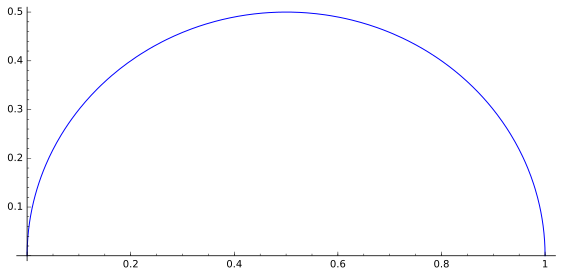
\includegraphics[width=0.5\textwidth]{circle.pdf}
  \caption{Circle with center at $x=1$}
\end{figure}
\item Indeed, $y = \sqrt{1/4 - (x-1/2)^2}$.
\item In this case it does since for $f(0)-f(1) = f'(1/2)(0-1)$ since $f'(1/2)=0$.
    \end{enumerate}
\end{soln}
\vspace{1in}




\end{document}








